\chapter{Anwendungsszenarien}
\section{Text-Mining, Natural Language Processing}
\section{Soziale Netze}
Unter dem Begriff Sozialem Netz versteht man eine Menge an Teilnehmern, häufig sind dies natürliche Personen, und verschiedenen Arten an Relationen zwischen diesen. Das durch die Beziehungen gebildete Netz lässt sich problemlos als Graph darstellen, indem die Teilnehmer als Knoten des Graphen dargestellt und die Beziehungen auf die Kanten abgebildet werden.

\begin{figure}
	\caption{Auschnitt aus Facebooks Socail-Graph: Checkin \cite{facebookTao}}
	\label{fig:fbCheckin}
	\centering
	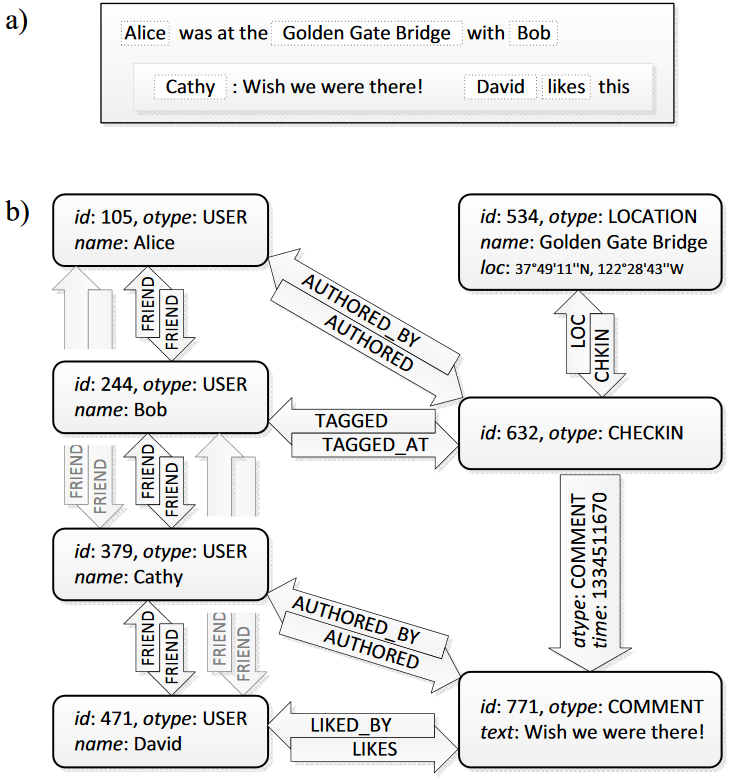
\includegraphics[width=0.7\textwidth]{images/facebook_checkin.png}
\end{figure}

Abbildung~\ref{fig:fbCheckin} zeigt beispielhaft wie ein Teil des Sozialen Netzes von Facebook aussieht. Anhand solcher Einträge wird für jeden einzelnen Nutzer eine personalisierte Startseite in Echtzeit erzeugt, dementsprechend wichtig ist ein performanter Datenzugriff. Um den Anforderungen gerecht zu werden hat Facebook eine eigene Graph-ähnliche API namens TAO entwickelt, welche den Datenbankzugriff effizient steuert. TAO stellt minimale Create/Update/Delete-Kommandos für Knoten und Kanten bereit. Der Großteil der Datenbankzugriffe ist allerdings lesend, folgende Querys sind möglich \cite{facebookTao}:
\begin{itemize}
	\item Alle Assoziation eines Typs zu einem Knoten
	\item Anzahl der Assoziationen eines Typs an einem Knoten
	\item Alle Nachbarn bis zur Tiefe n über eine bestimmte Assoziation
\end{itemize}
Dies ist ausreichend um mittels Verfahren wie Zentralitätsberechnung, Dichte und Cliquenanalyse für den Nutzer relevante Beiträge zu bestimmen \cite{sozialeNetzwerkanalyse}.


\section{Betrugserkennung}
Graph Datenbanken werden in e-commerce benutzt um die Betrug zu vermeiden. In Graph Datenbanken ist es möglich das Suchen der verdächtigen Pattern einzustellen - die entsprechenden Prüfungen, die mit den verschiedenen Triggern verbunden sind. Diese Triggern lassen sich die Probleme identifizieren, bevor als der ernschafte Schaden getroffen wird. Triggern können aus die nächste Ereignissen besteht werden: Einloggen in System, Registrierung einer neuen Bankkarte oder Bestellung der Waren.
\begin{figure}
	\caption{Serien von den Transaktionen}
	\label{fig:Trs}
	\centering
	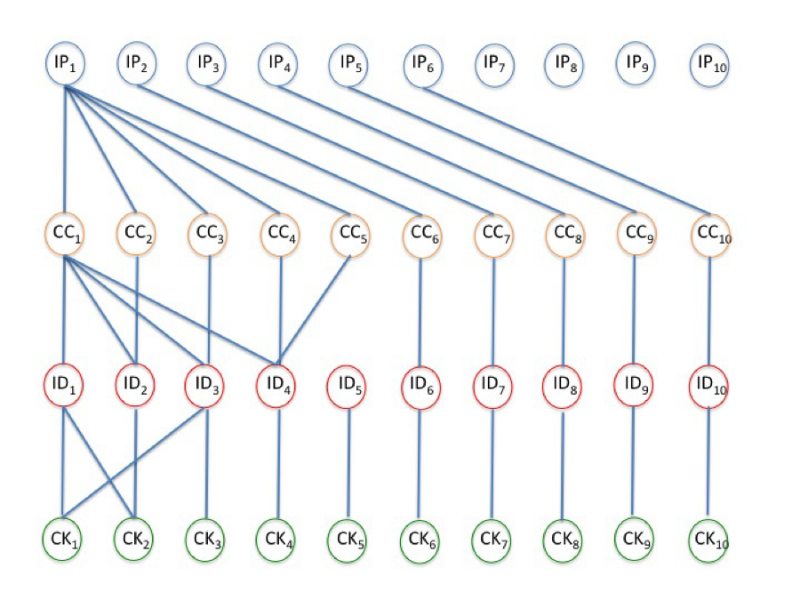
\includegraphics[width=0.7\textwidth]{images/Betrugserkennung.png}
\end{figure}

Auf der Abbildung~\ref{fig:Trs} sind die Transaktionsserien von den verschiedenen IP Adressen gezeigt. (IP(x) - IP Adresse, CC(x) - die Nummer der Kreditkarte, ID(x) - der Identifikator vom Nutzer, CK(x) - das Cookie, das im Systeme enthält). In diesem Beispiel ist es vermutlich, dass IP(1) von den Betrugen benutzt wird, denn vom IP(1) sind viele Transaktionen mit den unterschidliechen Kreditkarten durchgeführt, und eine Karte wurde von mehreren Nutzer benutzt, einige der auch mehr als eine Cookie besitzen. 
Graph Datenbanken sind die idealerweise Lösung der Bedrohungsentdeckung, die mit dem Finanzsicherheit in Netz verbunden sind, denn die Aktivität der Angreifern entspricht in jedem Fall zu einigen Pattern, und wenn sie rechtzeitig erkannt werden, können die möglichen Schaden minimiert werden.

\section{Empfehlungs-Engine}
Die Empfehlungsalgorithmen stellen die Verbindung zwischen den Leuten und den Dingen ein (die Waren, Dienstleistungen, Media-content) - alles, was relevant in diesem Bereich ist, wo diese Empfehlungsalgorithmen verwendet werden. Die Beziehungen werden basiert auf Benutzerverhalten. (Einkaufen, Bewertung, usw)
Die Effektivität der Empfehlungen hängt von dem Verstehen der Beziehungen zwischen Dingen ab und auch die Verbindung -qualität und -stärke. Diese Struktur ist am besten in Form von den attributierten Graphen vorgestellt. Die Anfragen in den Graphen sind meistens lokal, weil ihr Startpunkte ein oder einige identifizierte Objekte ist, und die weitere Suche ist in der Nähe von dieser Objekten durcgefürt.
Eine der ersten Empfehlungsalgorithmen war das System des Internet-Handels Amazon. Ein weiterentwickeltes Empfehlungsalgorithmus wurde von Google hergestellt. In diesem System war erstmal das Sammlungsverfahren der Nutzersinformationen verwendet worden, das cookies während der Besuchung der Suchmaschinen-Website benutzt wird und aufgrund der Suchensergebnisse wurde das Profil für jeden Nutzer aufgebaut.

\section{Verkehrsnetze}
\section{Stammdatenmanagement}
Stammdaten heißen die Daten, die kritisch wichtig für die Geschäftstransaktionen. Die Basisdaten enthält die Daten über die Benutzer, Einkäuferen, Produkten, Lieferanten, Abteilungen, Webseiten, usw. In den größen Organisationen sind solche Daten stark verteilt und heterogen nach den Formaten, Qualität und Zugangsmitteln. Das Stammdatenmanagement enthält die Identifizierung, Löschung, Speicherung und entsprechend Datenverwaltung. Das Stammdatenmanagement soll an der Veränderung der Oraganisationsstruktur, Verschmelzung von den Organisationen, Änderung der Geschäftsregeln usw. angepasst werden. Graph Datenbanken werden gut für die Modelirung, Speicherung, und Anfragen zu den Basismetadaten und Stammdatenmodellen gepasst werden. 

